\begin{figure}[tb]
    \centering
    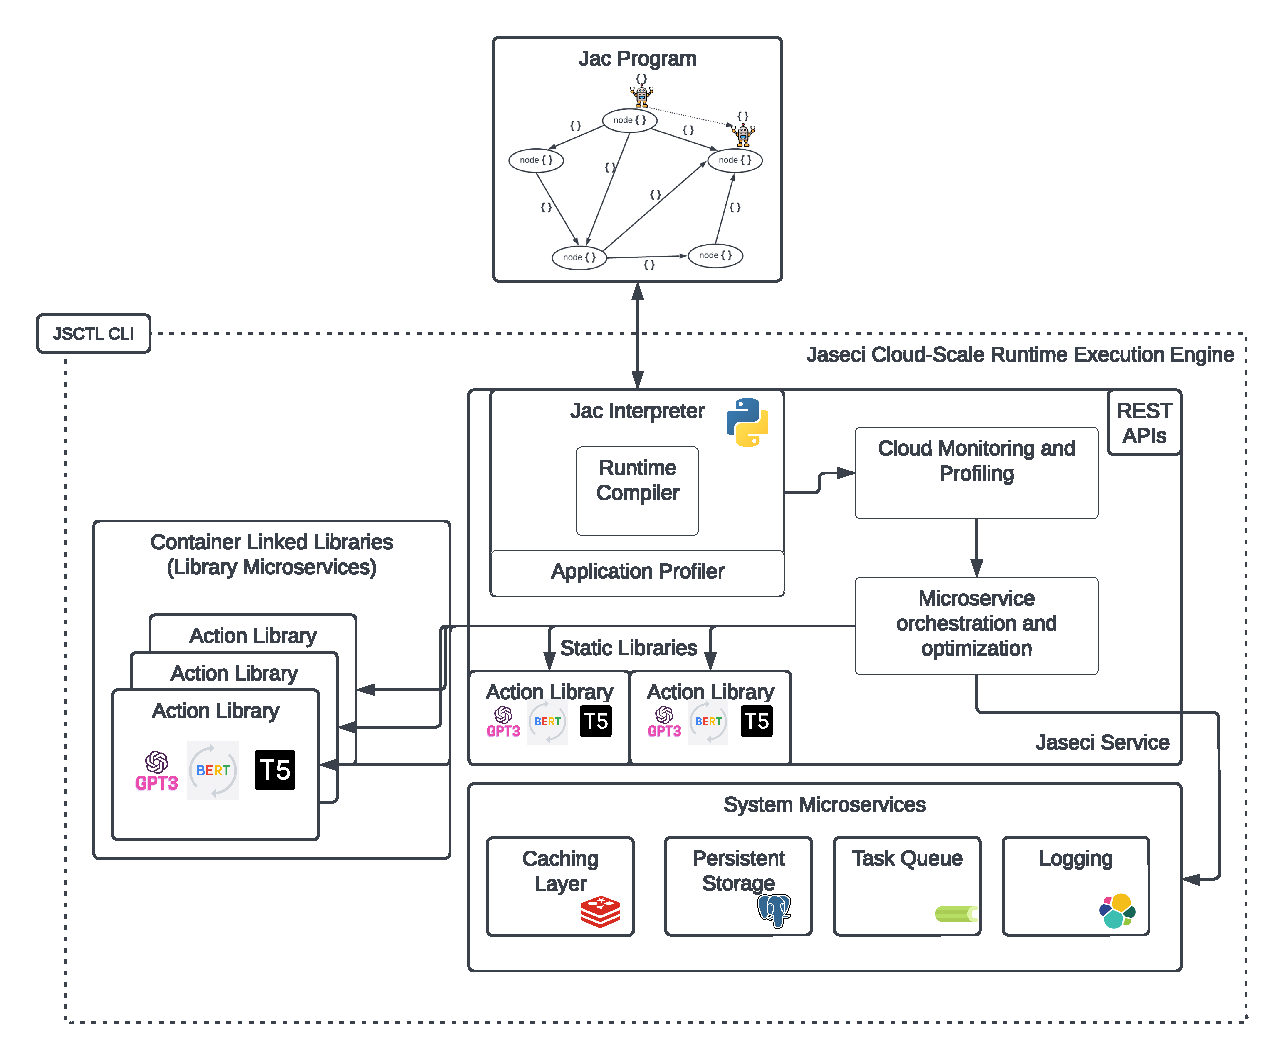
\includegraphics[width=\linewidth]{figures/jaseci_arch.pdf}
    \caption{The architecture of the Jaseci diffuse runtime execution. The runtime stack includes and combines information from interpreter level profiling, cloud monitoring and profiling, microservice orchestrator and optimizer. Container linked libraries are also depicted. }
    \label{fig:benefit2}
\end{figure}

Jaseci's cloud-scale runtime engine presents a higher level abstraction of the software stack.
The \emph{diffuse} runtime engine subsumes responsibility not only for the optimization of program code, but also the orchestration, configuration, and optimization of constituent micro services and the full cloud compute stack.
Duties such as container formation, microservice scaling, scheduling and optimization are automated by the runtime.
For example, as shown in Figure~\ref{fig:benefit2}c Jaseci introduces the concept of \textbf{container linked libraries} to complement traditional notions of statically and dynamically linked libraries.
From the programmers perspective, they need not know whether a call to a library is fused with the running programming instance or a remote call to a microservice somewhere in a cluster.
The decisioning of what \emph{should} be a microservice and what should be statically in the programs object scope is made automatically and seamlessly by the Jaseci \textbf{microservice orchestration engine}.
Underlying in-cluster microservices are encapsulated and hidden with this abstraction.
With the runtime having full visibility and control over the diffuse application, high complexity runtime decisions and heuristics such as autoscaling is brought under the purview of the runtime software stack, relieving the need of manual configuration.
With this Jaseci runtime, a single frontend engineer was able to implement the full ZeroShotBot~\cite{zsb-website} application (which uses a number of transformer neural networks) without writing a single line of traditional `backend' code.
This implementation currently support tens of thousands of queries a day across about $\sim$12 business customers with tens of thousands of individual end users in a single production environment.